\documentclass[../zhang_thesis.tex]{subfiles}
\begin{document}

\chapter{Methodology}

%%%%%%%%%%%%%%%%%%%%%%%%%%%%%%%%%%%%%%%%%%%%%%%%%%%%%%%%%%%%%%%

\section{Battery Model}

As discussed in the previous section, this thesis considers the electrical-circuit battery model proposed by Chen and Rinc\'on-Mora~\cite{chen06} and shown in \autoref{fig:batt_model}. The left portion of the circuit models the capacity, SOC, and runtime, while the right portion models the transient i-v characteristics.  For convenience, the model is designed so that the SOC of the battery equals the voltage $V_\text{SOC}$, in volts. The parameters $C_\text{cap}$ and $R_{sd}$ are assumed constant
for a given battery and determine the capacity and self-discharge rate of the battery. The other parameters are all nonlinear functions of $V_\text{SOC}$ and determine the transient i-v response as well as the open-circuit voltage $V_\text{OC}$. From a typical TCL PL-383562 polymer lithium-ion battery, Chen and Rinc\'on-Mora extracted these parameters and fit them to curves, obtaining
\begin{gather}
    R_s(V_\text{SOC}) = 0.1562 e^{-24.37 V_\text{SOC}} + 0.07446 \label{eq:nl_param_1} \\
    R_{ts}(V_\text{SOC}) = 0.3208 e^{-29.14 V_\text{SOC}} + 0.04669 \\
    C_{ts}(V_\text{SOC}) = -752.9 e^{-13.51 V_\text{SOC}} + 703.6 \\
    R_{tl}(V_\text{SOC}) = 6.603 e^{-155.2 V_\text{SOC}} + 0.04984 \\
    C_{tl}(V_\text{SOC}) = -6056 e^{-27.12 V_\text{SOC}} + 4475 \\
    V_\text{OC}(V_\text{SOC}) = -1.031 e^{-35 V_\text{SOC}} + 3.685 + 0.2156 V_\text{SOC} - 0.1178 V_\text{SOC}^2 + 0.3201 V_\text{SOC}^3 \label{eq:nl_param_6}
\end{gather}
The resistance and capacitance parameters shown above are approximately constant for $\text{SOC}>0.2$ and change exponentially for $\text{SOC}<0.2$. The open-circuit voltage also changes exponentially for $\text{SOC}<0.2$ but is approximately linear for $\text{SOC}>0.2$. Note that the capacitances $C_{ts}$ and $C_{tl}$ are negative for SOC values close to zero, which is both unrealistic according to the experimental data collected by Chen and Rin\'on-Mora and problematic mathematically. To solve this, a lower bound was placed on the $V_\text{SOC}$ input to the capacitance functions. Thus, for inputs below some threshold value $v_T$, the capacitances are adjusted to their value at that threshold, producing
\begin{align}
    \hat{C}_{ts}{V_\text{SOC}} &= \begin{cases}
        C_{ts}(V_\text{SOC}), & V_\text{SOC} \ge v_T \\
        C_{ts}(v_T), & V_\text{SOC} < v_T
        \end{cases} \label{eq:Cts_thres} \\
    \hat{C}_{tl}{V_\text{SOC}} &= \begin{cases}
        C_{tl}(V_\text{SOC}), & V_\text{SOC} \ge v_T \\
        C_{tl}(v_T), & V_\text{SOC} < v_T \label{eq:Ctl_thres}
        \end{cases}
\end{align}
The threshold $v_T$ was chosen based on the experimental data of Chen and Rin\'on-Mora, specifically so that the threshold capacitance values are approximately equal to the lowest such values measured by them. A threshold of $v_T=0.015$~V accomplishes this goal.

\begin{figure}[ht]
\centering
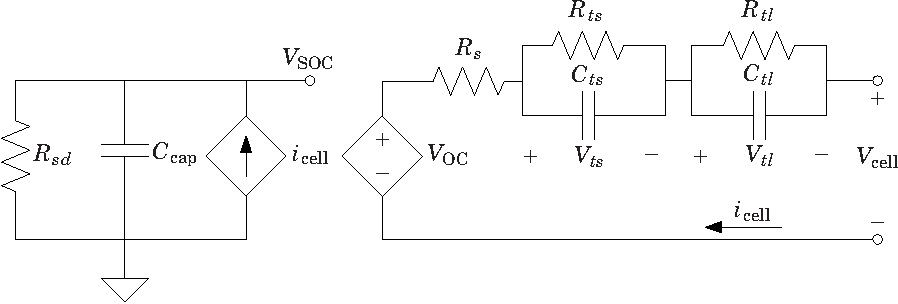
\includegraphics[width=0.9\textwidth]{batt_model}
\caption{Battery model for simulation. [From paper, will redo later]}
\label{fig:batt_model}
\end{figure}

This study used the nonlinear parameters given by Chen and Rinc\'on-Mora for the implementation of a battery using their battery model in Matlab. In addition, the thresholding defined in \autorefs{eq:Cts_thres} and \ref{eq:Ctl_thres} was used with $v_T=0.015$~V. The other, constant parameters were chosen to produce a capacity of 1~Ah and a self-discharge rate of 4\% per month. To do so, the capacitance $C_\text{cap}$ is calculated to hold the desired capacity when $V_\text{SOC}=1$~V, and then the resistance $R_{sd}$ is set
to produce the desired self-discharge rate. For a given capacity of $C^\dag$ in Ah, $C_\text{cap}$ needs to be
\begin{equation}
    C_\text{cap} = \frac{Q}{V_\text{SOC}} = \frac{C^\dag}{1~\text{V}} = 3600 C^\dag \,[\text{F}].
\end{equation}
Then, the resistance $R_{sd}$ is chosen so that the time constant $\tau=RC$ results in the desired drop of $\xi=0.04$ over $T=1$~month as follows
\begin{gather}
    V(t) = V_0 e^{-T/\tau} = V_0 (1-\xi) \\
    \tau = -T/\ln(1-\xi) = -2592000/\ln 0.96 \,[\text{s}].
\end{gather}
Then, $R_{sd}=\tau/C_\text{cap}$. Thus, the parameters are $C_\text{cap}=3600$~F and $R_{sd}=17.6376~\mathrm{k}\Omega$.


%To better determine the necessity of nonlinear filtering for thus system, it is useful to determine the degree of nonlinearity. Recent work in quantizing the degree of nonlinearity was conducted by

\section{Simulation Setup}

\begin{figure}[ht]
\centering
% This file is generated by the MATLAB m-file laprint.m. It can be included
% into LaTeX documents using the packages graphicx, color and psfrag.
% It is accompanied by a postscript file. A sample LaTeX file is:
%    \documentclass{article}\usepackage{graphicx,color,psfrag}
%    \begin{document}% This file is generated by the MATLAB m-file laprint.m. It can be included
% into LaTeX documents using the packages graphicx, color and psfrag.
% It is accompanied by a postscript file. A sample LaTeX file is:
%    \documentclass{article}\usepackage{graphicx,color,psfrag}
%    \begin{document}% This file is generated by the MATLAB m-file laprint.m. It can be included
% into LaTeX documents using the packages graphicx, color and psfrag.
% It is accompanied by a postscript file. A sample LaTeX file is:
%    \documentclass{article}\usepackage{graphicx,color,psfrag}
%    \begin{document}\input{batt_load_exp}\end{document}
% See http://www.mathworks.de/matlabcentral/fileexchange/loadFile.do?objectId=4638
% for recent versions of laprint.m.
%
% created by:           LaPrint version 3.16 (13.9.2004)
% created on:           18-Feb-2014 21:34:20
% eps bounding box:     15 cm x 8.1771 cm
% comment:              
%
\begin{psfrags}%
\psfragscanon%
%
% text strings:
\psfrag{s05}[t][t]{\color[rgb]{0,0,0}\setlength{\tabcolsep}{0pt}\begin{tabular}{c}Time (seconds)\end{tabular}}%
\psfrag{s06}[b][b]{\color[rgb]{0,0,0}\setlength{\tabcolsep}{0pt}\begin{tabular}{c}$\mathrm{V_{cell}}$\end{tabular}}%
\psfrag{s07}[b][b]{\color[rgb]{0,0,0}\setlength{\tabcolsep}{0pt}\begin{tabular}{c}Time Series Plot:$\mathrm{V_{cell}}$\end{tabular}}%
\psfrag{s08}[t][t]{\color[rgb]{0,0,0}\setlength{\tabcolsep}{0pt}\begin{tabular}{c}Time (seconds)\end{tabular}}%
\psfrag{s09}[b][b]{\color[rgb]{0,0,0}\setlength{\tabcolsep}{0pt}\begin{tabular}{c}$\mathrm{i_{cell}}$\end{tabular}}%
\psfrag{s10}[b][b]{\color[rgb]{0,0,0}\setlength{\tabcolsep}{0pt}\begin{tabular}{c}Time Series Plot:$\mathrm{i_{cell}}$\end{tabular}}%
\psfrag{s11}[t][t]{\color[rgb]{0,0,0}\setlength{\tabcolsep}{0pt}\begin{tabular}{c}Time (seconds)\end{tabular}}%
\psfrag{s12}[b][b]{\color[rgb]{0,0,0}\setlength{\tabcolsep}{0pt}\begin{tabular}{c}$R_L$\end{tabular}}%
%
% xticklabels:
\psfrag{x01}[t][t]{0}%
\psfrag{x02}[t][t]{5000}%
\psfrag{x03}[t][t]{10000}%
\psfrag{x04}[t][t]{15000}%
\psfrag{x05}[t][t]{0}%
\psfrag{x06}[t][t]{5000}%
\psfrag{x07}[t][t]{10000}%
\psfrag{x08}[t][t]{15000}%
\psfrag{x09}[t][t]{0}%
\psfrag{x10}[t][t]{5000}%
\psfrag{x11}[t][t]{10000}%
\psfrag{x12}[t][t]{15000}%
%
% yticklabels:
\psfrag{v01}[r][r]{-6}%
\psfrag{v02}[r][r]{-4}%
\psfrag{v03}[r][r]{-2}%
\psfrag{v04}[r][r]{0}%
\psfrag{v05}[r][r]{2}%
\psfrag{v06}[r][r]{4}%
\psfrag{v07}[r][r]{6}%
\psfrag{v08}[r][r]{-1}%
\psfrag{v09}[r][r]{-0.5}%
\psfrag{v10}[r][r]{0}%
\psfrag{v11}[r][r]{0.5}%
\psfrag{v12}[r][r]{1}%
\psfrag{v13}[r][r]{2}%
\psfrag{v14}[r][r]{2.5}%
\psfrag{v15}[r][r]{3}%
\psfrag{v16}[r][r]{3.5}%
\psfrag{v17}[r][r]{4}%
\psfrag{v18}[r][r]{4.5}%
%
% Figure:
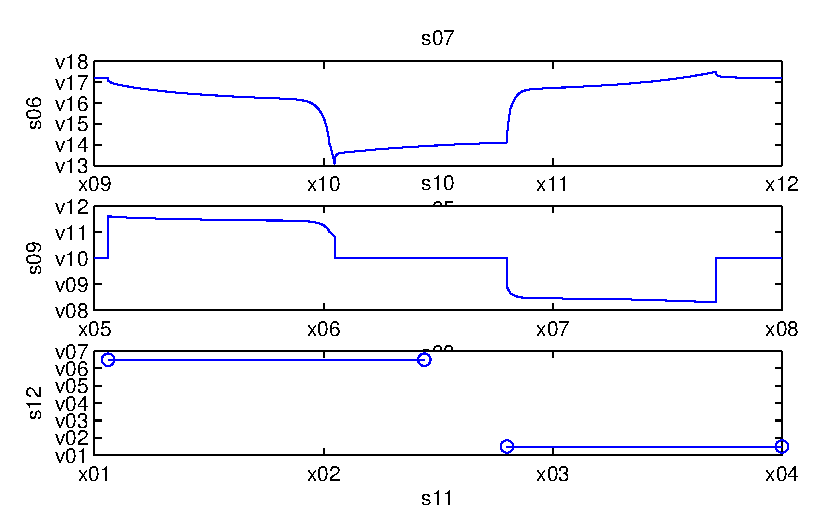
\includegraphics[width=12cm]{batt_load_exp.eps}%
\end{psfrags}%
%
% End batt_load_exp.tex
\end{document}
% See http://www.mathworks.de/matlabcentral/fileexchange/loadFile.do?objectId=4638
% for recent versions of laprint.m.
%
% created by:           LaPrint version 3.16 (13.9.2004)
% created on:           18-Feb-2014 21:34:20
% eps bounding box:     15 cm x 8.1771 cm
% comment:              
%
\begin{psfrags}%
\psfragscanon%
%
% text strings:
\psfrag{s05}[t][t]{\color[rgb]{0,0,0}\setlength{\tabcolsep}{0pt}\begin{tabular}{c}Time (seconds)\end{tabular}}%
\psfrag{s06}[b][b]{\color[rgb]{0,0,0}\setlength{\tabcolsep}{0pt}\begin{tabular}{c}$\mathrm{V_{cell}}$\end{tabular}}%
\psfrag{s07}[b][b]{\color[rgb]{0,0,0}\setlength{\tabcolsep}{0pt}\begin{tabular}{c}Time Series Plot:$\mathrm{V_{cell}}$\end{tabular}}%
\psfrag{s08}[t][t]{\color[rgb]{0,0,0}\setlength{\tabcolsep}{0pt}\begin{tabular}{c}Time (seconds)\end{tabular}}%
\psfrag{s09}[b][b]{\color[rgb]{0,0,0}\setlength{\tabcolsep}{0pt}\begin{tabular}{c}$\mathrm{i_{cell}}$\end{tabular}}%
\psfrag{s10}[b][b]{\color[rgb]{0,0,0}\setlength{\tabcolsep}{0pt}\begin{tabular}{c}Time Series Plot:$\mathrm{i_{cell}}$\end{tabular}}%
\psfrag{s11}[t][t]{\color[rgb]{0,0,0}\setlength{\tabcolsep}{0pt}\begin{tabular}{c}Time (seconds)\end{tabular}}%
\psfrag{s12}[b][b]{\color[rgb]{0,0,0}\setlength{\tabcolsep}{0pt}\begin{tabular}{c}$R_L$\end{tabular}}%
%
% xticklabels:
\psfrag{x01}[t][t]{0}%
\psfrag{x02}[t][t]{5000}%
\psfrag{x03}[t][t]{10000}%
\psfrag{x04}[t][t]{15000}%
\psfrag{x05}[t][t]{0}%
\psfrag{x06}[t][t]{5000}%
\psfrag{x07}[t][t]{10000}%
\psfrag{x08}[t][t]{15000}%
\psfrag{x09}[t][t]{0}%
\psfrag{x10}[t][t]{5000}%
\psfrag{x11}[t][t]{10000}%
\psfrag{x12}[t][t]{15000}%
%
% yticklabels:
\psfrag{v01}[r][r]{-6}%
\psfrag{v02}[r][r]{-4}%
\psfrag{v03}[r][r]{-2}%
\psfrag{v04}[r][r]{0}%
\psfrag{v05}[r][r]{2}%
\psfrag{v06}[r][r]{4}%
\psfrag{v07}[r][r]{6}%
\psfrag{v08}[r][r]{-1}%
\psfrag{v09}[r][r]{-0.5}%
\psfrag{v10}[r][r]{0}%
\psfrag{v11}[r][r]{0.5}%
\psfrag{v12}[r][r]{1}%
\psfrag{v13}[r][r]{2}%
\psfrag{v14}[r][r]{2.5}%
\psfrag{v15}[r][r]{3}%
\psfrag{v16}[r][r]{3.5}%
\psfrag{v17}[r][r]{4}%
\psfrag{v18}[r][r]{4.5}%
%
% Figure:
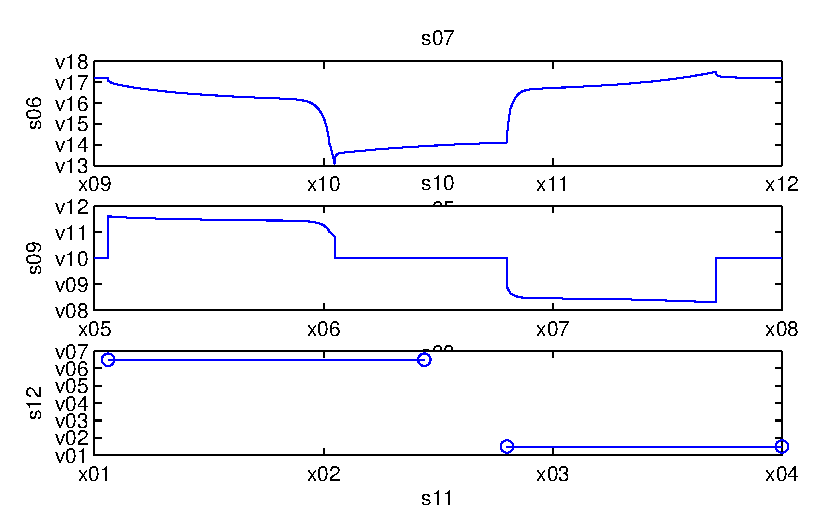
\includegraphics[width=12cm]{batt_load_exp.eps}%
\end{psfrags}%
%
% End batt_load_exp.tex
\end{document}
% See http://www.mathworks.de/matlabcentral/fileexchange/loadFile.do?objectId=4638
% for recent versions of laprint.m.
%
% created by:           LaPrint version 3.16 (13.9.2004)
% created on:           18-Feb-2014 21:34:20
% eps bounding box:     15 cm x 8.1771 cm
% comment:              
%
\begin{psfrags}%
\psfragscanon%
%
% text strings:
\psfrag{s05}[t][t]{\color[rgb]{0,0,0}\setlength{\tabcolsep}{0pt}\begin{tabular}{c}Time (seconds)\end{tabular}}%
\psfrag{s06}[b][b]{\color[rgb]{0,0,0}\setlength{\tabcolsep}{0pt}\begin{tabular}{c}$\mathrm{V_{cell}}$\end{tabular}}%
\psfrag{s07}[b][b]{\color[rgb]{0,0,0}\setlength{\tabcolsep}{0pt}\begin{tabular}{c}Time Series Plot:$\mathrm{V_{cell}}$\end{tabular}}%
\psfrag{s08}[t][t]{\color[rgb]{0,0,0}\setlength{\tabcolsep}{0pt}\begin{tabular}{c}Time (seconds)\end{tabular}}%
\psfrag{s09}[b][b]{\color[rgb]{0,0,0}\setlength{\tabcolsep}{0pt}\begin{tabular}{c}$\mathrm{i_{cell}}$\end{tabular}}%
\psfrag{s10}[b][b]{\color[rgb]{0,0,0}\setlength{\tabcolsep}{0pt}\begin{tabular}{c}Time Series Plot:$\mathrm{i_{cell}}$\end{tabular}}%
\psfrag{s11}[t][t]{\color[rgb]{0,0,0}\setlength{\tabcolsep}{0pt}\begin{tabular}{c}Time (seconds)\end{tabular}}%
\psfrag{s12}[b][b]{\color[rgb]{0,0,0}\setlength{\tabcolsep}{0pt}\begin{tabular}{c}$R_L$\end{tabular}}%
%
% xticklabels:
\psfrag{x01}[t][t]{0}%
\psfrag{x02}[t][t]{5000}%
\psfrag{x03}[t][t]{10000}%
\psfrag{x04}[t][t]{15000}%
\psfrag{x05}[t][t]{0}%
\psfrag{x06}[t][t]{5000}%
\psfrag{x07}[t][t]{10000}%
\psfrag{x08}[t][t]{15000}%
\psfrag{x09}[t][t]{0}%
\psfrag{x10}[t][t]{5000}%
\psfrag{x11}[t][t]{10000}%
\psfrag{x12}[t][t]{15000}%
%
% yticklabels:
\psfrag{v01}[r][r]{-6}%
\psfrag{v02}[r][r]{-4}%
\psfrag{v03}[r][r]{-2}%
\psfrag{v04}[r][r]{0}%
\psfrag{v05}[r][r]{2}%
\psfrag{v06}[r][r]{4}%
\psfrag{v07}[r][r]{6}%
\psfrag{v08}[r][r]{-1}%
\psfrag{v09}[r][r]{-0.5}%
\psfrag{v10}[r][r]{0}%
\psfrag{v11}[r][r]{0.5}%
\psfrag{v12}[r][r]{1}%
\psfrag{v13}[r][r]{2}%
\psfrag{v14}[r][r]{2.5}%
\psfrag{v15}[r][r]{3}%
\psfrag{v16}[r][r]{3.5}%
\psfrag{v17}[r][r]{4}%
\psfrag{v18}[r][r]{4.5}%
%
% Figure:
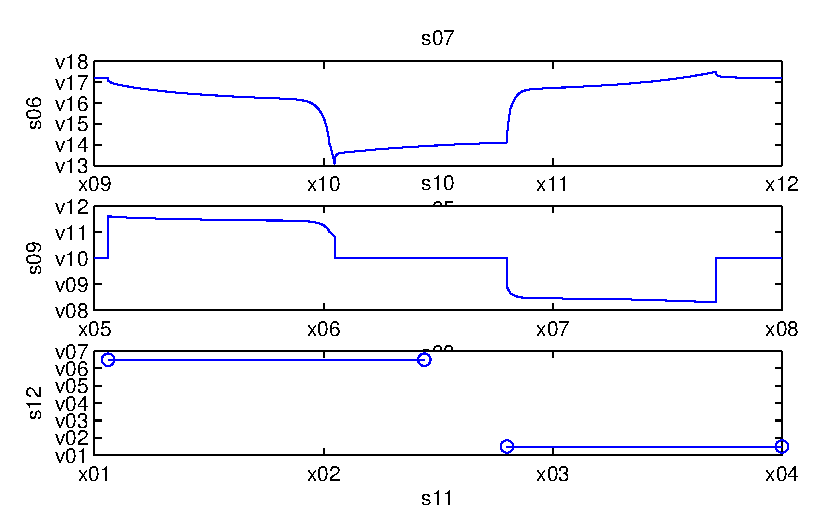
\includegraphics[width=12cm]{batt_load_exp.eps}%
\end{psfrags}%
%
% End batt_load_exp.tex

\caption{Test of loading battery with resistive load and charging using negative resistance.}
\label{fig:batt_load_exp}
\end{figure}

\section{Filter Implementations}

%As was seen in the last section, the degree of nonlinearity of the battery model necessitates the use of a nonlinear filter. However, for SOC$>0.2$, the dynamics behave approximately linearly, because the resistance and capacitance parameters are approximately constant. Since the battery operates in this ``linear'' region for the majority of the time, it is useful to compare the performance of a linear filter to the nonlinear filters discussed in \autoref{sec:nl_filt}.

%In order to determine the necessity of incorporating the nonlinear relationship between $V_\text{SOC}$ and $V_\text{OC}$ in the filter design, the linearized right-hand circuit with $V_\text{SOC}=0.6$~V and the left-hand circuit were processed by a Kalman filter in each iteration and in that order, with the nonlinearity calculated implicitly.
% the left-hand circuit along with the right-hand circuit linearized at $V_\text{SOC}=0.6$~V were consecutively processed by the Kalman filter in each itera


\end{document}
